\documentclass[aspectration=169]{beamer}
\usepackage{amsfonts,amsmath,oldgerm,graphicx,epstopdf}
\usepackage{booktabs}
\usepackage[euler]{textgreek}
\epstopdfsetup{outdir=illustration/}
\setbeamertemplate{caption}{\color{maincolor}Fig. \color{darkgray} \raggedright\insertcaption\par}
\newcommand{\B}{\textcolor{maincolor}{\textbullet}}

\usetheme{sintef}

% TODO: NMR del pirazolo estere (?)
% TODO: aggiungere sintesi dei monomeri ed introduzione sul legante
% TODO: check coerenza rese tesi e presentazione

% \newcommand{\testcolor}[1]{\colorbox{#1}{\textcolor{#1}{test}}~\texttt{#1}}

\usefonttheme[onlymath]{serif}

\titlebackground*{assets/background}

\newcommand{\hrefcol}[2]{\textcolor{cyan}{\href{#1}{#2}}}

\title{\large{Investigation of the synthesis of a new \\ pyrazole dicarboxylate ligand for the construction of new MOFs}}
\course{\vspace{0.2cm}\tiny Relatrice: Prof. Lucia Carlucci \\ \vspace{-0.2cm} Co-relatore: Pierluigi Mercandelli}
\subtitle{Laurea Triennale in Chimica}
\author{\href{stefano.marton@studenti.unimi.it}{Stefano Marton}}
\IDnumber{962848}

\begin{document}
\maketitle

\section{Sintesi del legante pirazolico}

\setlength{\columnsep}{0.2cm}
\begin{frame}{Perché leganti con funzionitá pirazoliche?}
	% Buongiorno a tutti, sono contento oggi di presentare il mio lavoro di tesi
	% con titolo "Investigation of the synthesis of a new pyrazole dicarboxylate ligand for the
	% construction of new MOFs" che ho avuto modo di svolgere presso il
	% laboratorio della professa Carlucci.
	% Il lavoro da me svolto si suddivide principalmente in 2 parti, di cui la principale é dedicata allo sviluppo della sintesi del legante pirazolico,
	% mentre la seconda sull'esplorazione della reattivitá elettrochimica di leganti dichetonici.
	% L'idea del progetto di tesi nasce dall'interesse verso la funzionilitá pirazolica all'interno di leganti per la
	% costruzione di MOFs. L'anello pirazolico permette di ottenere una serie di
	% caratteristiche desiderabili quali rigiditá strutturale, resistenza termica e
	% soprattutto, nel caso in cui non agisca come sito di coordinazione é in grado di
	% instaurare interazioni intermolecolari che rendono possibile l'adsorbimento
	% specifico di sostanze quali gas o acqua all'interno del MOF. Questa proprietá
	% risulta ampiamente documentata in letteratura e i primi passi del progetto si
	% muovono proprio a partire da li. In figura riporto il legante utilizzato
	% all'interno del MOF-303 ottenuto dal professor Yaghi e un legante recentemente studiato all'interno del
	% gruppo della professoressa Carlucci. A partire da questa situazione si é
	% inizialmente pensato di convertire il legante rappresentato a sinistra ad una
	% funzionalitá pirazolica.
	\begin{columns}
		\hspace{1cm}
		\begin{column}{0.3\textwidth}
			\begin{itemize}
				\item Rigiditá strutturale
				\item Resistenza termica
				\item Legami idrogeno
			\end{itemize}
		\end{column}
		\hspace{-0.5cm}
		\begin{column}{0.7\textwidth}
			\begin{figure}[h]
				\includegraphics[width=8cm,keepaspectratio]{illustration/drawing2.pdf}
			\end{figure}
		\end{column}
	\end{columns}
\end{frame}

\subsection{Addizione diretta di idrazina al dichetone}
% Per procedere alla conversione si ripreso il lavoro giá svolto sul legante
% dichetonico di cui riporto qui l'approccio retrosintetico. Si procede con una
% condensazione di Claisen incrociata a partire da materiali facilmente reperibili
% commercialmente, si effettua un'addizione diretta di idrazina ai gruppi
% chetonici che porta al prodotto pirazolico che viene successivamente sottoposto
% ad idrolisi.
\begin{frame}{Addizione diretta di idrazina al dichetone}
	\framesubtitle{Retrosintesi}
	\begin{figure}[h]
		\centering
		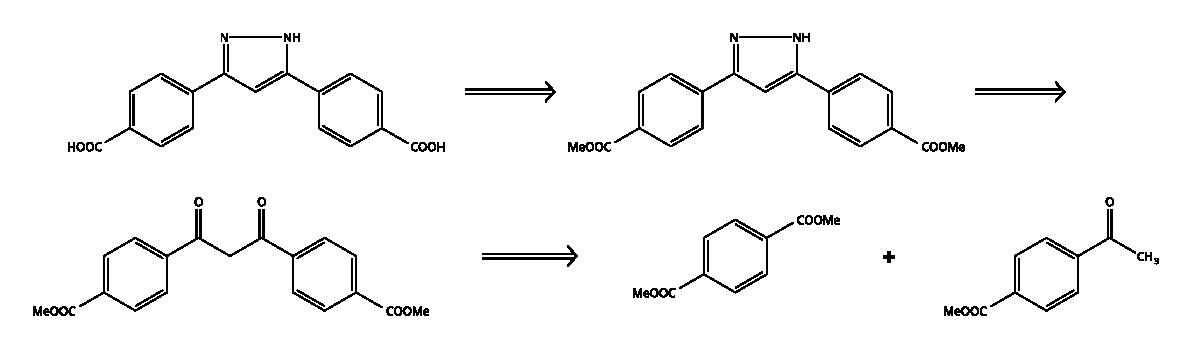
\includegraphics[width=14cm,height=8cm,keepaspectratio]{../Structures/pyr-retro.eps}
		\caption{Approccio retrosintetico sfruttando l'addizione diretta di idrazina}
	\end{figure}
\end{frame}

% La claisen incrociata avviene con rese soddisfacenti in condizioni
% relativamente comode, il processo di purificazione composto da lavaggi con %
% TODO: cosa?
% Permette di ottenere un prodotto con elevato grado di purezza
% adeguato a procedere con la sintesi. A partire dall'intermedio ottenuto si puó
% procedere con il passaggio chiave della sintesi del legante, cioé la formazione
% dell'anello pirazolico.
\begin{frame}{Reazione di Claisen incrociata}
	\centering
	\framesubtitle{Primo passaggio sintetico}
	\begin{figure}[h!]
		\centering
		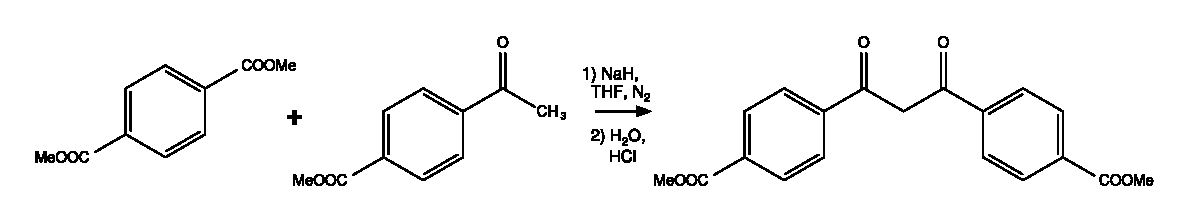
\includegraphics[width=13cm,keepaspectratio]{illustration/claisen.eps}
	\end{figure}
	\vspace{0.5cm}
	\B \ Atmosfera inerte \hspace{1cm} \B \ Prodotto puro \hspace{1cm} \B \ Resa 92\%
\end{frame}

% Il passaggio critico é insito proprio nella formazione dell'anello che porta
% con se numerose criticitá.
% Le rese della reazione sono poco soddisfacenti, il prodotto ottenuto non ha un buon grado di purezza e richiede conseguentemente
% una fase di purificazione.

\begin{frame}{Addizione diretta di idrazina al dichetone}
	\centering
	\framesubtitle{Passaggio chiave}
	\begin{figure}[h]
		\includegraphics[width=13cm,height=8cm,keepaspectratio]{../Structures/pyrazole-form.eps}
		\caption{Reazione chiave di formazione dell'anello pirazolico}
	\end{figure}
	\vspace{0.5cm}
	\B \ Difficile recupero del prodotto \hspace{0.6cm} \B \ Prodotto non puro \hspace{0.6cm} \B \ Resa \(<\) 25\%
\end{frame}

% Sono state effettuate una serie di prove che comprendono variazione di
% solvente, temperatura e catalizzatori della reazione per cercare di ottimizzare i risultati.
% La solubilitá dell'intermedio dichetonico é minima nella maggior parte dei solventi se non
% quelli altobollenti, che come mostrato in tabella portano ad un leggero aumento
% di resa, seguito, inevitabilmente da numerosi problemi di recupero del prodotto.
% In particolare la resa maggiore é stata ottenuta utilizzando come solvente il DMSO che é sostanzialmente l'unico solvente che permette al reagente iniziale di solubilizzarsi, tuttavia la reazione é seguita da un workup particolarmente dispendioso. Infatti é necessario procedere ad un altissima diluzione in acqua, raffreddamento e successiva centrifugazione per recuperare il prodotto formato. La fase di cristallizzazione, che per quanto osservato risulta il miglior metodo di purificazione per il prodotto in questione, diventa inapplicabile in quanto il prodotto é estramamente solubile in DMSO e non precipita.

\begin{frame}{Addizione diretta di idrazina al dichetone}
	\framesubtitle{Condizioni di Reazione e Recupero del Prodotto}
	\begin{columns}
		\hspace{1cm}
		\begin{column}{0.5\textwidth}
			Condizioni di reazione
			\begin{itemize}
				\small
				\item Solvente e solubilitá
				\item Temperatura
				\item Tempo di reazione
				\item Catalisi acida e basica
				\item Equivalenti di idrazina
			\end{itemize}
			\vspace{0.2cm}
			Recupero del prodotto
			\begin{itemize}
				\item Colonna Cromatografica
				\item Ricristallizzazione
				\item Soxhlet
			\end{itemize}
			\vspace*{-1cm}
		\end{column}
		\hspace{-3cm}
		\begin{column}{0.5\textwidth}
			\begin{footnotesize}
				\begin{center}
					\begin{tabular}{cccc}
						\toprule
						{Solvente} & T [K] & t [h] & Resa [\%]     \\
						\midrule
						DMF        & 403   & 17    & \(< 10\)      \\
						DMSO       & 433   & 24    & \(\simeq 25\) \\
						EtOH       & 351   & 4     & \(-\)         \\
						EtOH       & 351   & 17    & \(< 5\)       \\
						THF        & 339   & 36    & \(-\)         \\
						\bottomrule
					\end{tabular}
				\end{center}
			\end{footnotesize}
		\end{column}
	\end{columns}
\end{frame}

\begin{frame}{Idrolisi del diestere}
	\centering
	\framesubtitle{Ultima reazione del path sintetico}
	\begin{figure}[h!]
		\centering
		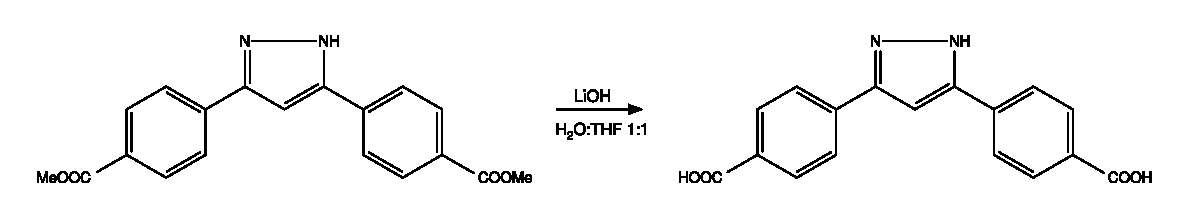
\includegraphics[width=10cm,keepaspectratio]{illustration/idrolisi.eps}
	\end{figure}
	\vspace{0.5cm}
	\B \ Difficile recupero del prodotto \hspace{0.6cm} \B \ Prodotto di partenza variabile
\end{frame}

\subsection{Addizione coniugata di idrazina all'\textalpha,\textbeta -insaturo}

% Alla luce delle criticitá incontrate con l'addizione diretta di idrazina al dichetone si é riflettuto su una possibile via alternativa, in particolare si é verificata la possibilitá di ottenere l'anello pirazolico a partire dal composto alfa-beta insaturo corrispondente.
% Di questo approccio sintetico alternivo viene riportata di seguito l'approccio retrosintetico che quindi procede attraverso una prima condensazione aldolica mista, seguita dall'addizione coniugata di idrazina e successiva idrolisi.

\begin{frame}{Addizione coniugata di idrazina all'\textalpha,\textbeta -insaturo}
	\framesubtitle{Retrosintesi}
	\begin{figure}[h!]
		\centering
		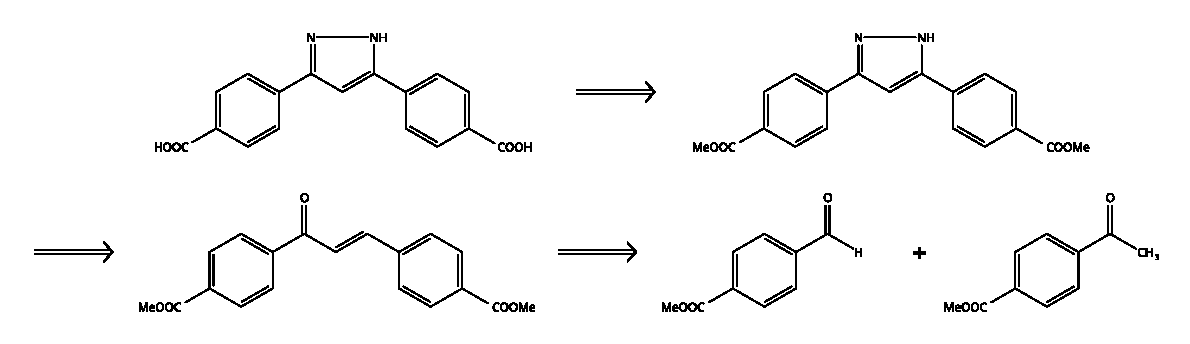
\includegraphics[width=13cm,height=8cm,keepaspectratio]{../Structures/pyrazole-retro-alt.eps}
		\caption{Approccio retrosintetico sfruttando l'addizione coniugata di idrazina}
	\end{figure}
\end{frame}

\begin{frame}{Condensazione aldolica mista}
	\framesubtitle{Primo passaggio sintetico}
	\centering
	\begin{figure}[h]
		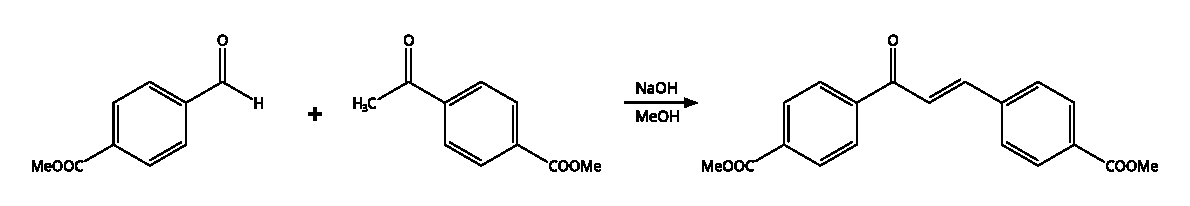
\includegraphics[width=13cm,height=8cm,keepaspectratio]{illustration/aldolica.eps}
	\end{figure}
	\vspace{0.5cm}
	\B \ Tecnicamente facile \ \hspace{1cm} \B \ Prodotto puro \hspace{1cm} \B \ Resa 94\%
\end{frame}

\begin{frame}{Addizione coniugata di idrazina all'\textalpha,\textbeta -insaturo}
	\framesubtitle{Passaggio chiave}
	\centering
	\begin{figure}[h]
		\centering
		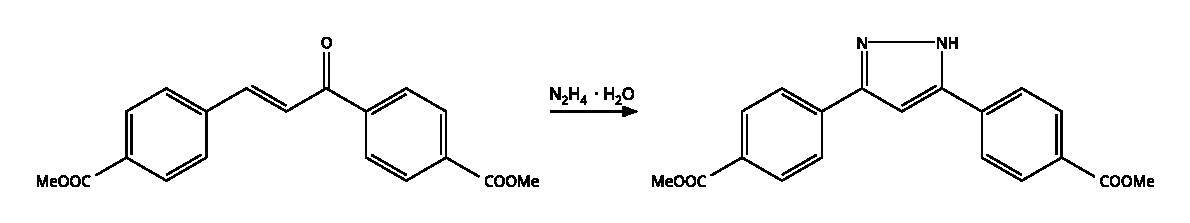
\includegraphics[width=13cm,height=8cm,keepaspectratio]{../Structures/pyrazole-form-alt.eps}
	\end{figure}
	\vspace{0.5cm}
	\B \ Non si osserva formazione di prodotto
\end{frame}

\begin{frame}{Addizione diretta di idrazina al dichetone}
	\framesubtitle{Condizioni di Reazione e Recupero del Prodotto}
	\begin{columns}
		\hspace{1cm}
		\begin{column}{0.5\textwidth}
			Condizioni di reazione
			\begin{itemize}
				\item Solvente e solubilitá
				\item Catalisi acida e basica
				\item Temperatura
				\item Tempo di reazione
				\item Microonde
			\end{itemize}
		\end{column}
		\hspace{-3cm}
		\begin{column}{0.5\textwidth}
			\begin{footnotesize}
				\begin{center}
					\begin{tabular}{cccc}
						\toprule
						{Solvente} & T [K]   & t [h] & Resa [\%] \\
						\midrule
						AcOH       & \(363\) & 3     & \(-\)     \\
						AcOH       & \(391\) & 17    & \(-\)     \\
						MeOH + HCl & \(351\) & 5     & \(-\)     \\
						MeOH + Py  & \(351\) & 5     & \(-\)     \\
						EtOH       & RT      & 5     & (?)       \\
						\bottomrule
					\end{tabular}
				\end{center}
			\end{footnotesize}
		\end{column}
	\end{columns}
\end{frame}

\begin{frame}{Addizione diretta di idrazina al dichetone}
	\framesubtitle{Intermedio idrazonico}
	\begin{figure}[h!]
		\centering
		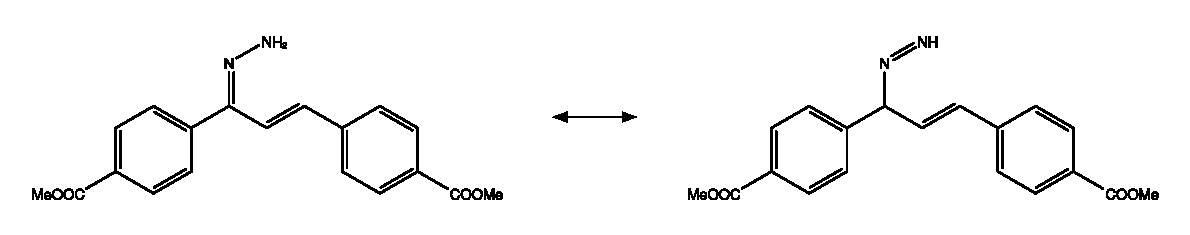
\includegraphics[width=13cm,keepaspectratio]{../Structures/idrazone.eps}
		\caption{Strutture di risonanza dell'intermedio idrazonico}
	\end{figure}
\end{frame}

\begin{frame}{Caratterizzazione}
	\centering
	\framesubtitle{NMR dell'intermedio idrazonico}
	\vspace{-1cm}
	\begin{columns}
		\begin{column}{0.55\textwidth}
			\begin{figure}[h!]
				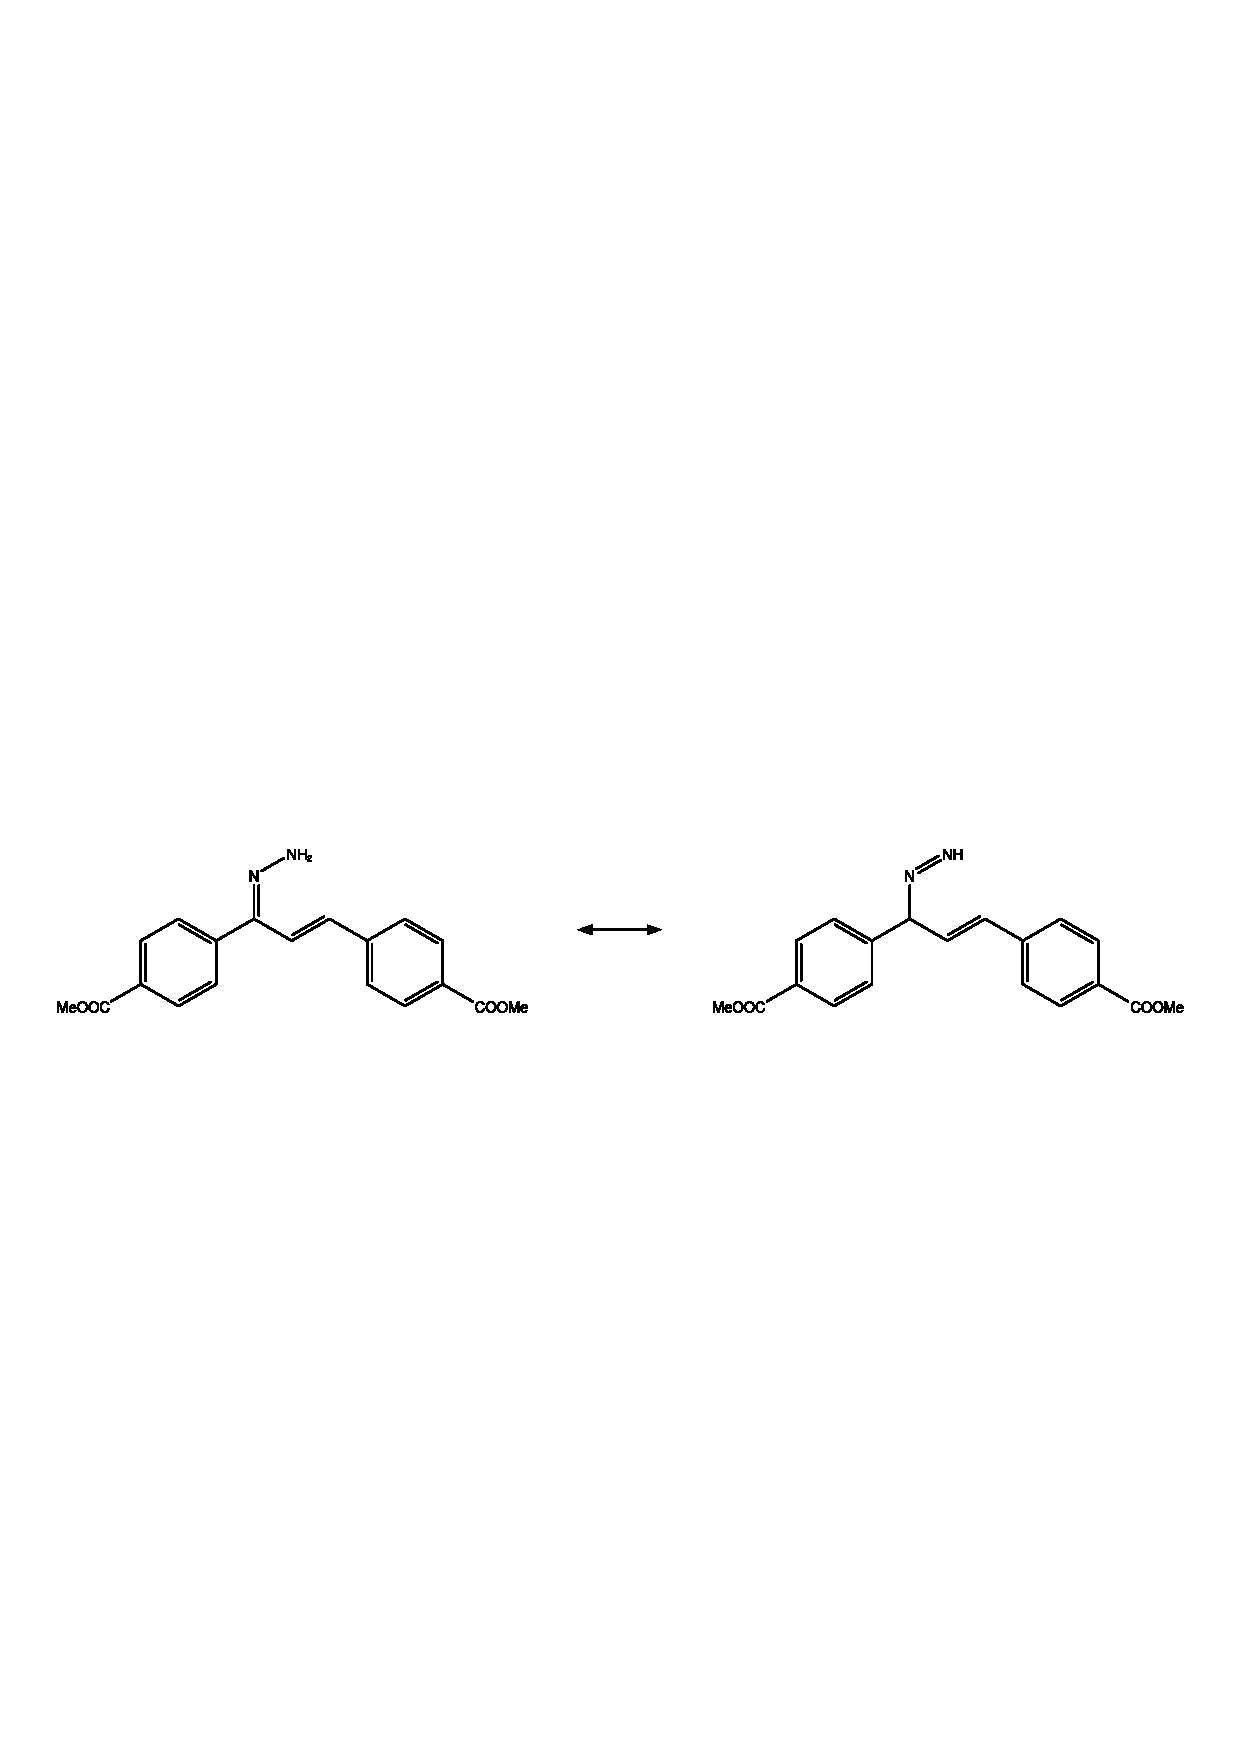
\includegraphics[width=8cm,keepaspectratio]{../Spectra/nmr/idrazone.pdf}
			\end{figure}
		\end{column}
		\begin{column}{0.55\textwidth}
			\begin{figure}[h!]
				\includegraphics[width=8cm,keepaspectratio]{../Spectra/nmr/idrazonenoesy.pdf}
			\end{figure}

			\hspace{2cm}
		\end{column}
	\end{columns}
\end{frame}

\section{Caratterizzazione elettrochimica di leganti dichetonici}

\begin{frame}{Perché elettrochimica?}
	\framesubtitle{Background}
	\begin{columns}
		\begin{column}{0.5\textwidth}
			\begin{columns}
				\begin{column}{0.5\textwidth}
					\begin{figure}[h!]
						\centering
						\includegraphics[width=1.5cm,keepaspectratio]{illustration/monomero2.png}
						% \caption{Struttura del monomero}
					\end{figure}
					\vspace*{-0.5cm}
				\end{column}
				\hspace{-2cm}
				\begin{column}{0.5\textwidth}
					\begin{figure}[h!]
						\centering
						\includegraphics[width=2cm,keepaspectratio]{illustration/monomero1.png}
						% \caption{Struttura del monomero}
					\end{figure}
				\end{column}
			\end{columns}
			\begin{figure}[h!]
				\centering
				
\includegraphics[width=3.8cm,keepaspectratio]{illustration/mof.png}
				% \caption{Struttura del monomero}
			\end{figure}
			\vspace*{-1cm}
			\hspace{-1cm}
		\end{column}
		\vspace{-4cm}
		\begin{column}{0.5\textwidth}
			\vspace{-2cm}
			\begin{center}
				\begin{figure}[h!]
					\centering
					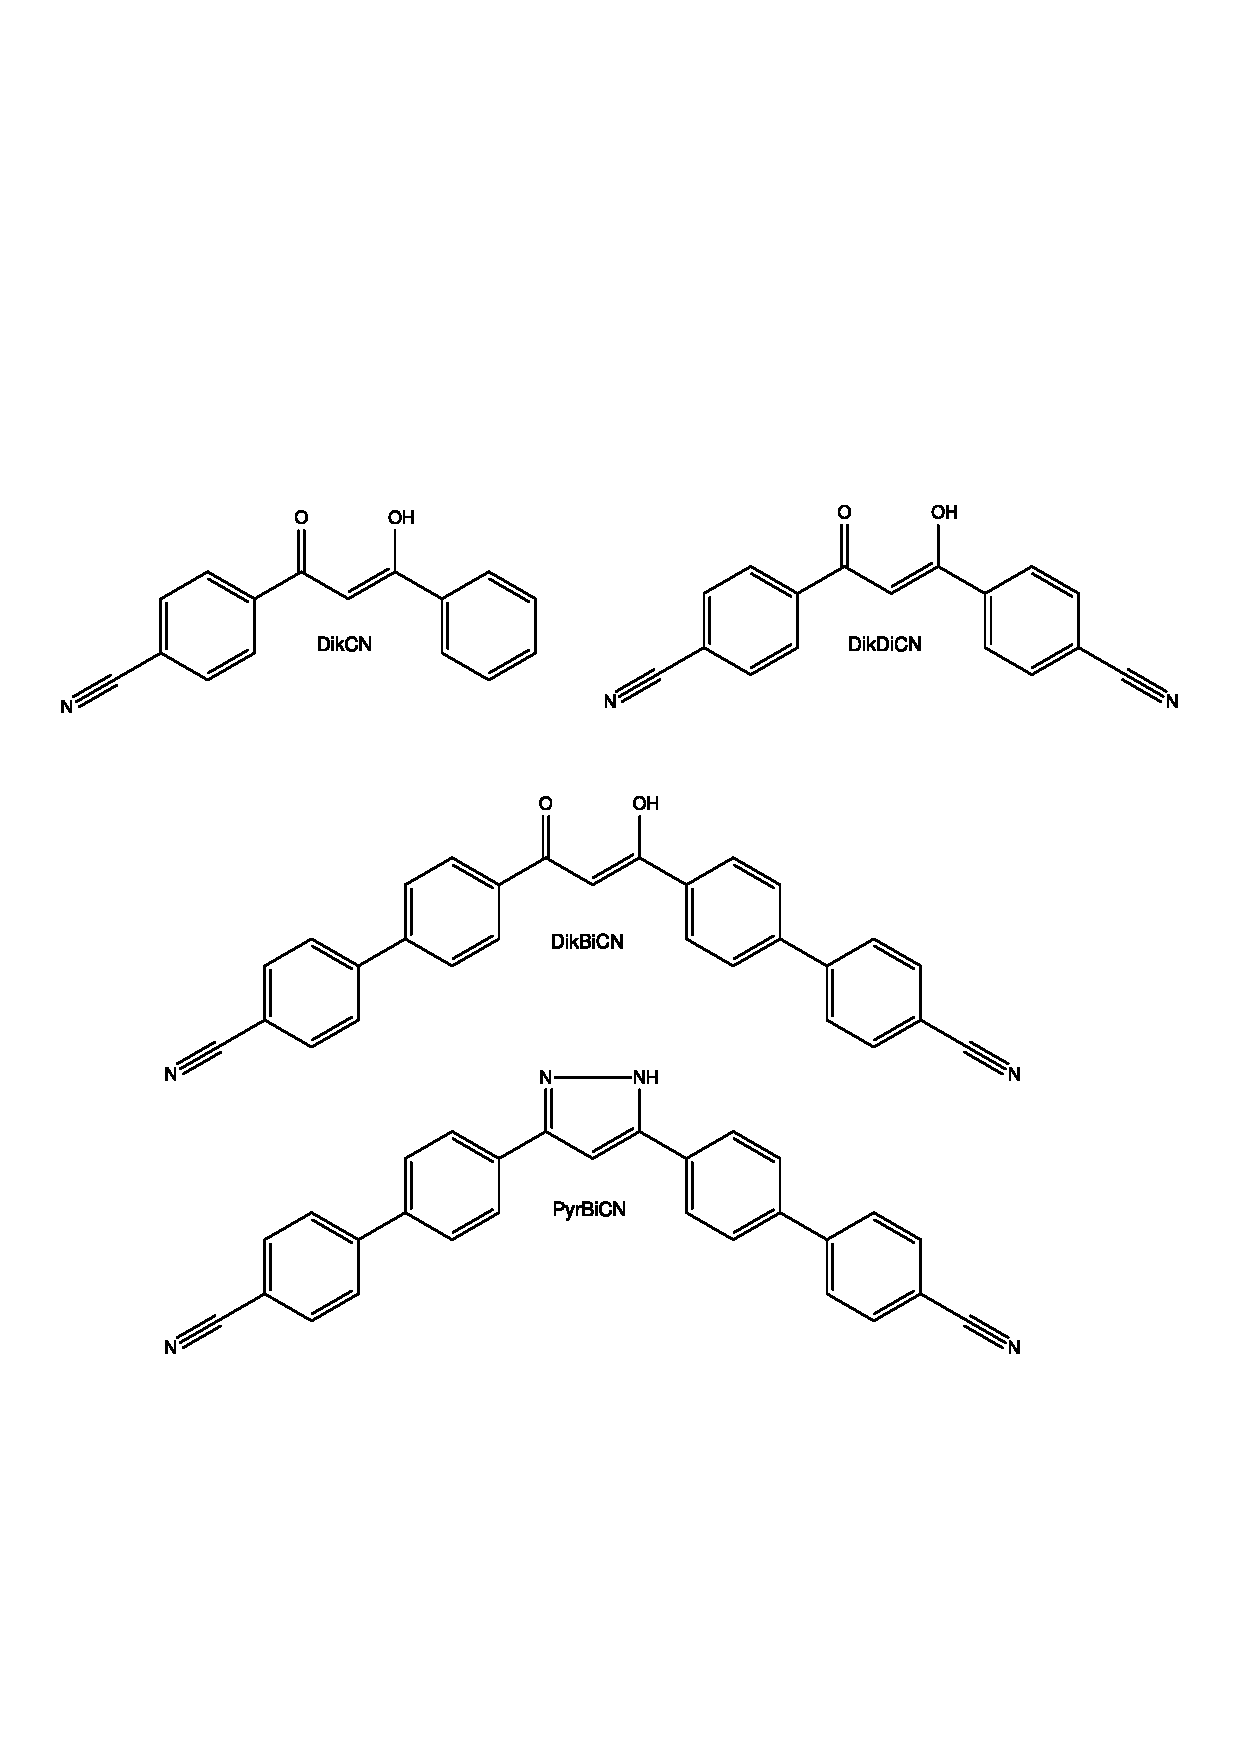
\includegraphics[width=5cm,keepaspectratio]{illustration/leganti.pdf}
					% \caption{Strutture dei leganti analizzati}
				\end{figure}
			\end{center}
		\end{column}
	\end{columns}
	\vspace{0.5cm}
	\centering
	\B \ Valutazione della reattivitá elettrochimica \hspace{1cm} \B \ Confronto nella famiglia di leganti
\end{frame}

% \begin{frame}{Caratterizzazione UV}
% 	\vspace{-0.5cm}
% 	\begin{columns}
% 		\hspace{-1cm}
% 		\begin{column}{0.5\textwidth}
% 			\begin{figure}[h!]
% 				\centering
% 				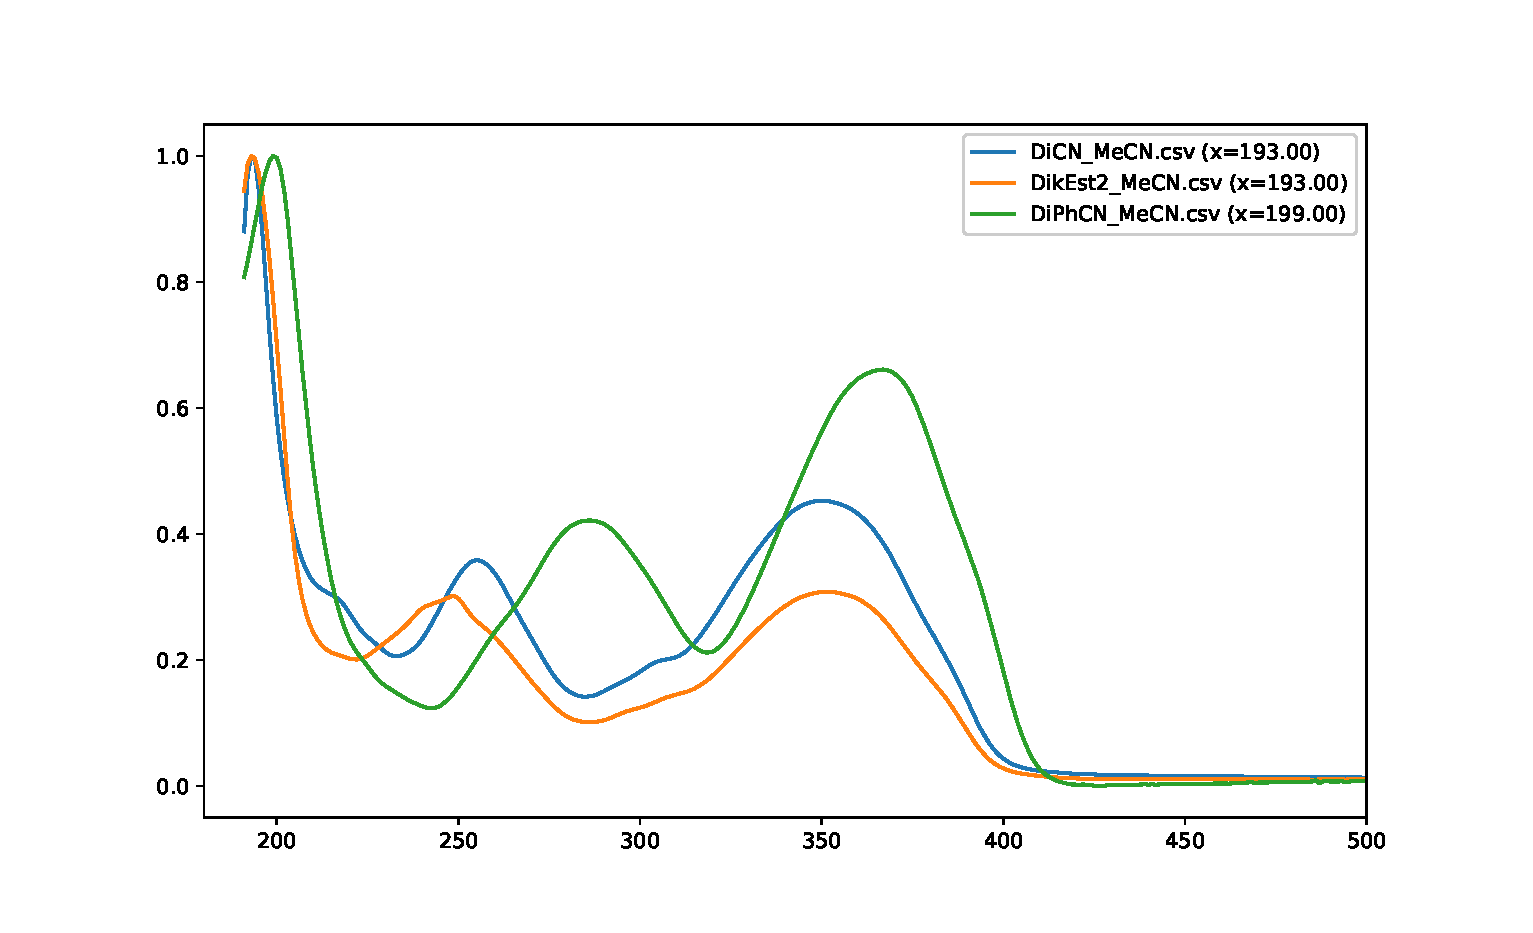
\includegraphics[width=8cm,keepaspectratio]{../Spectra/LegantiMeCN.eps}
% 				\vspace*{-8mm}
% 				\hspace*{3cm}
% 				\caption{UV in MeCN}
% 			\end{figure}
% 		\end{column}
% 		\hspace{-0.5cm}
% 		\begin{column}{0.5\textwidth}
% 			\begin{figure}[h!]
% 				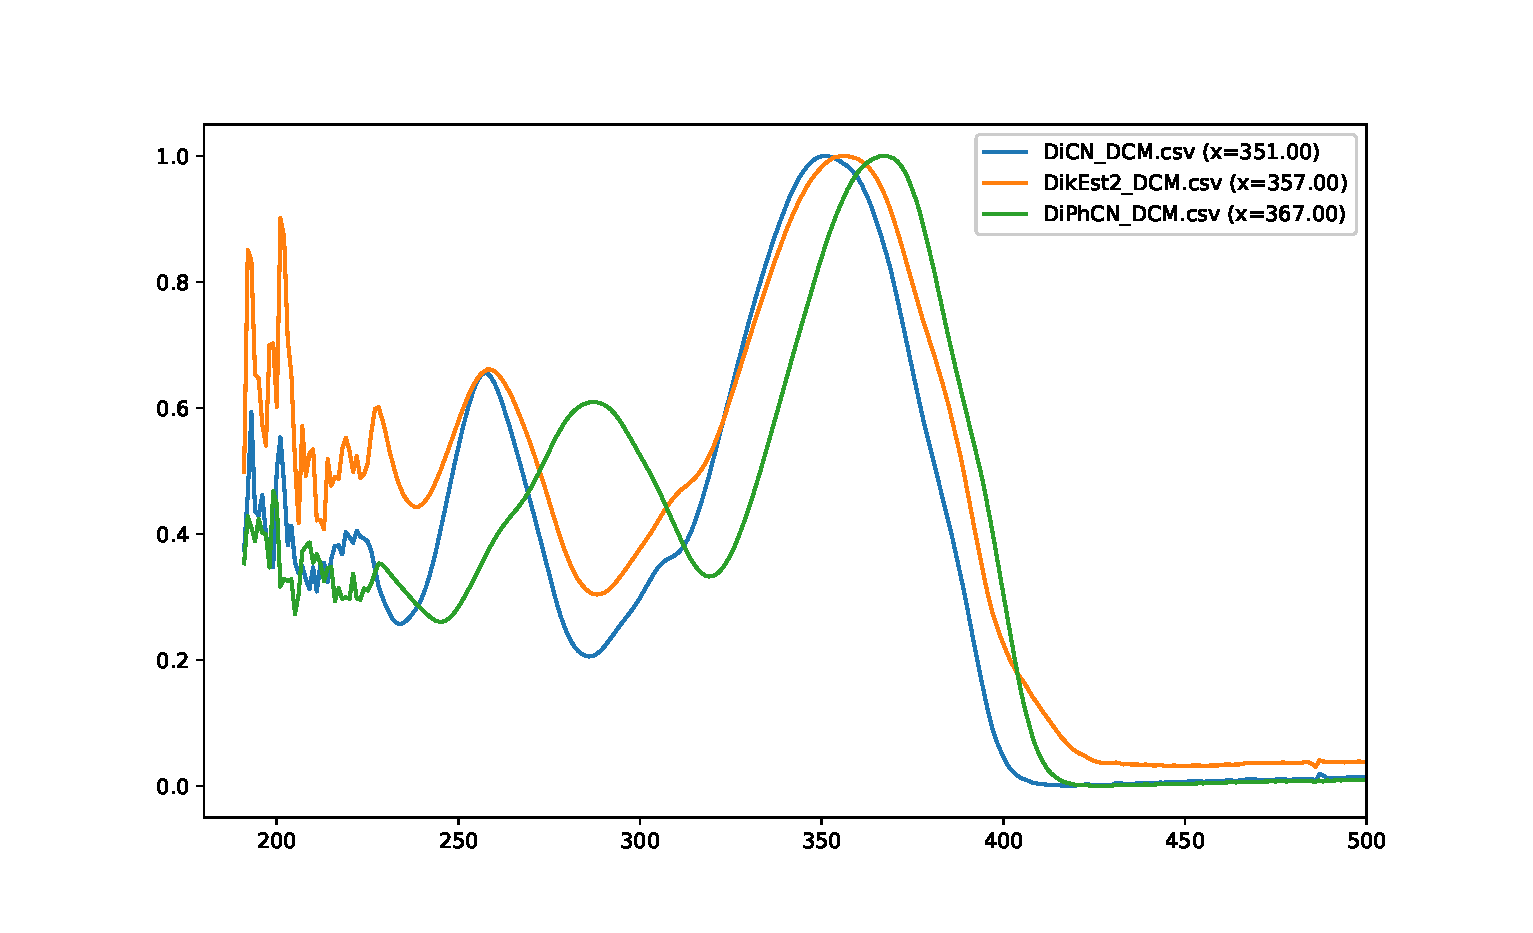
\includegraphics[width=8cm,keepaspectratio]{../Spectra/LegantiDCM.eps}
% 				\vspace*{-8mm}
% 				\caption{UV in MeCN}
% 			\end{figure}
% 		\end{column}
% 	\end{columns}
% \end{frame}

\subsection{Leganti}
\begin{frame}{Voltammetrica Ciclica}
	\centering
	\framesubtitle{Leganti}
	\begin{columns}
		\begin{column}{0.5\textwidth}
			\begin{figure}[h!]
				\vspace*{-0.5cm}
				\centering
				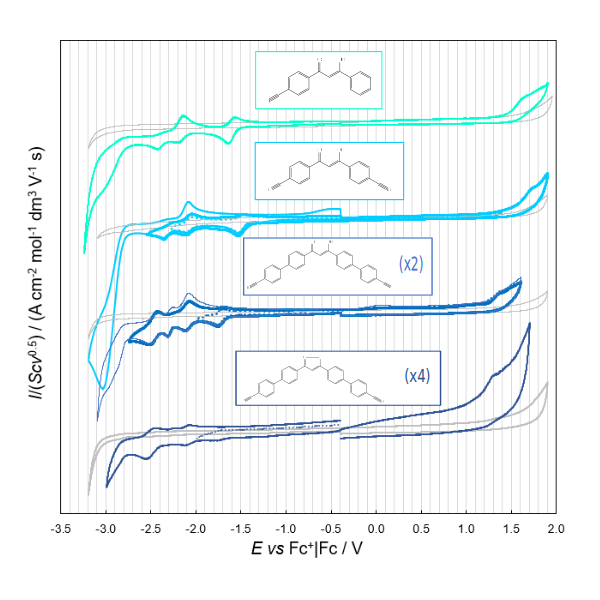
\includegraphics[width=7cm,keepaspectratio]{../Images/mussini/secondaimmagine.pdf}
			\end{figure}
		\end{column}
		\begin{column}{0.5\textwidth}
			\vspace*{-0.5cm}
			\begin{itemize}
				\item Effetto dei gruppi elettronattrattori sul primo evento di riduzione
				\item Effetto della distanza tra i gruppi
				\item Necessitá di analisi e confronti piú approfonditi
			\end{itemize}
		\end{column}
	\end{columns}
\end{frame}

\subsection{Monomeri}
\begin{frame}{Voltammetrica Ciclica}
	\framesubtitle{Monomeri}
	\begin{columns}
		\hspace{1cm}
		\begin{column}{0.5\textwidth}
			\begin{figure}[h!]
				\centering
				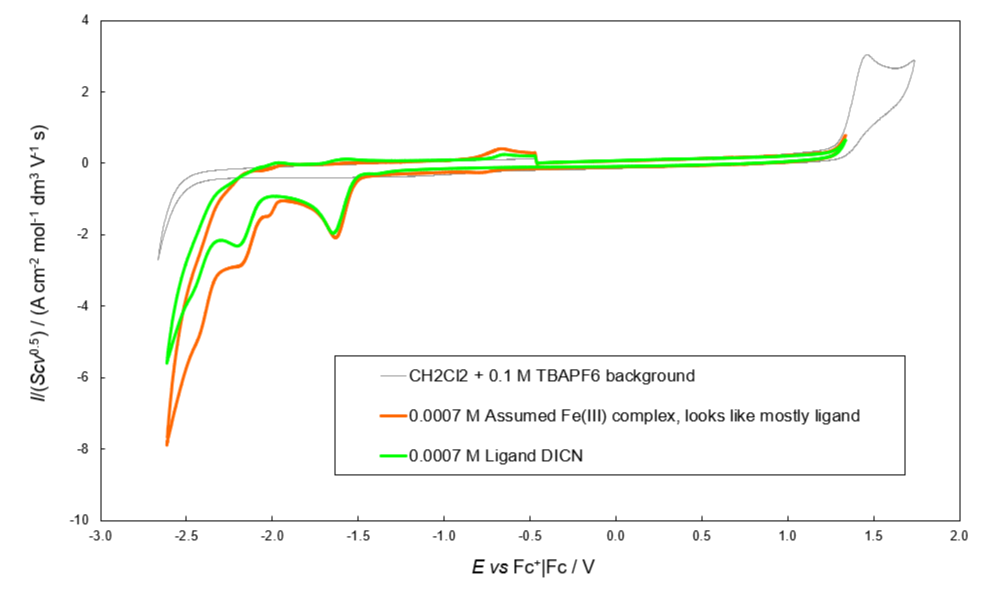
\includegraphics[width=7cm,keepaspectratio]{../Images/mussini/ultimafigura.pdf}
			\end{figure}
		\end{column}
		\begin{column}{0.5\textwidth}
			\begin{figure}[h!]
				\centering
				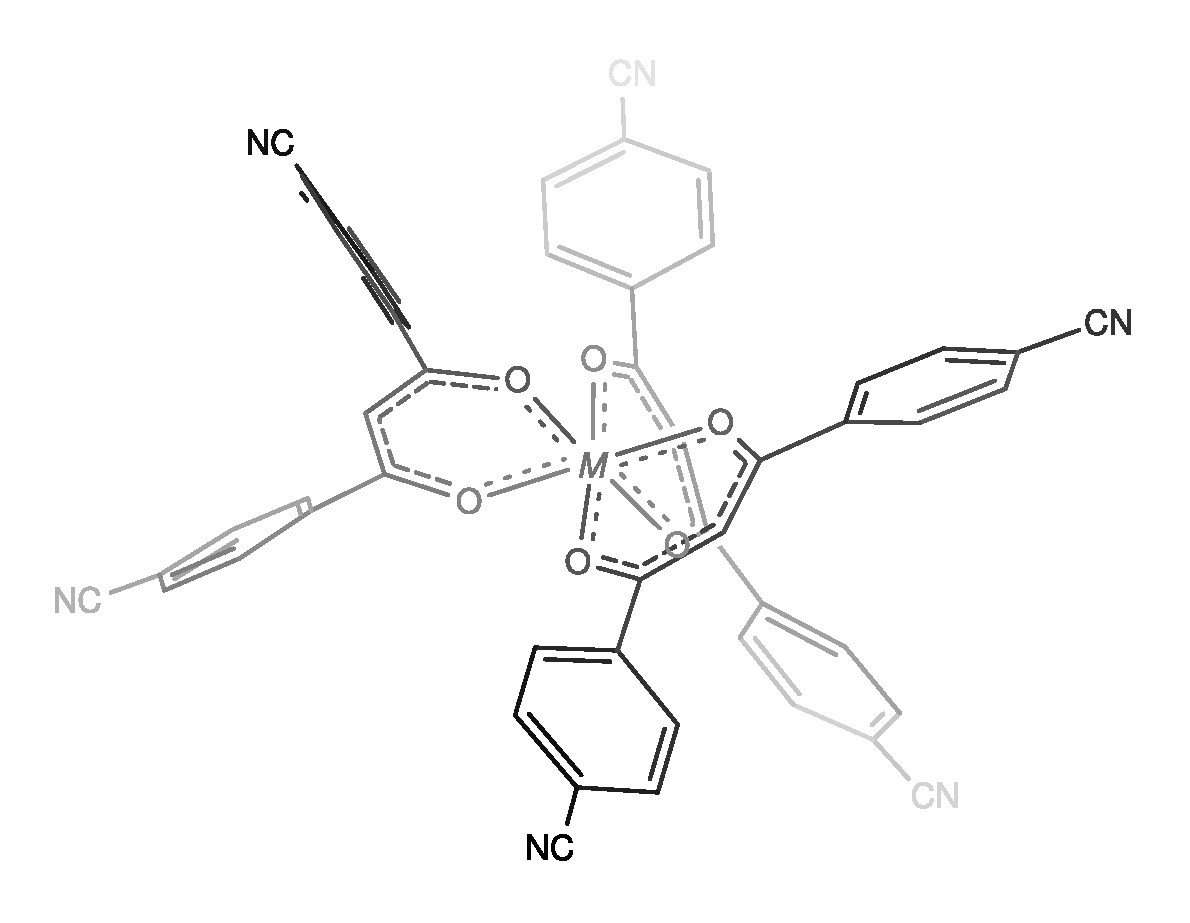
\includegraphics[width=3cm,keepaspectratio]{../Structures/monomero.eps}
				\caption{Struttura del monomero}
			\end{figure}
			\begin{itemize}
				\item Non si osserva significativa differenza
				\item Necessarie ulteriori indagini
			\end{itemize}
		\end{column}
	\end{columns}
	\vspace{0.5cm}
	\centering
\end{frame}

\begin{frame}{Conclusioni}
	\framesubtitle{Considerazioni e prospetti futuri}
	\B \ Diverse vie sintetiche per la sintesi del legante \\
	~~ \B \ Microonde


	\vspace{0.5cm}

	\B \ É stata preliminarmente esplorata la reattivitá elettrochimica
\end{frame}

\backmatter
\end{document}
